\documentclass{article}
\usepackage[x11names, rgb]{xcolor}
\usepackage[utf8]{inputenc}
\usepackage{tikz}
\usetikzlibrary{snakes,arrows,shapes}
\usepackage{amsmath}
%
%

%

%

\begin{document}
\pagestyle{empty}
%
%
%

\enlargethispage{100cm}
% Start of code
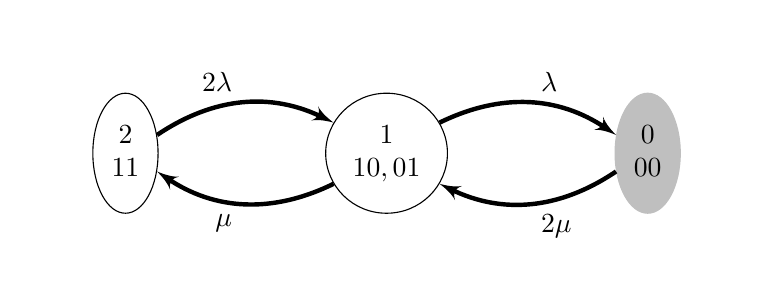
\begin{tikzpicture}[>=latex',line join=bevel,]
%%
\begin{scope}
  \pgfsetstrokecolor{black}
  \definecolor{strokecol}{rgb}{1.0,1.0,1.0};
  \pgfsetstrokecolor{strokecol}
  \draw (8bp,8bp) -- (8bp,97bp) -- (266bp,97bp) -- (266bp,8bp) -- cycle;
\end{scope}
  \node (1) at (137bp,52bp) [draw,ellipse] {$\begin{matrix}1 \\ 10,01 \end{matrix}$};
  \node (0) at (231bp,52bp) [draw=lightgray,fill=lightgray,ellipse] {$\begin{matrix}0 \\ 00 \end{matrix}$};
  \node (2) at (43bp,52bp) [draw,ellipse] {$\begin{matrix}2 \\ 11 \end{matrix}$};
  \draw [->,ultra thick] (1) to[bend left] node[auto] {$\lambda$} (0);
  \draw [->,ultra thick] (2) to[bend left] node[auto] {$2\lambda$} (1);
  \draw [->,ultra thick] (1) to[bend left] node[auto] {$\mu$} (2);
  \draw [->,ultra thick] (0) to[bend left] node[auto] {$2\mu$} (1);
%
\end{tikzpicture}
% End of code

%
\end{document}
%



